\documentclass{article}
\usepackage{ctex} % 排版中文文章
\usepackage{physics}
\usepackage{booktabs,tabularx,multicol,multirow} % 制作表格
\usepackage{appendix}
\usepackage{amsmath,amsthm,amssymb,amsfonts}    % 数学符号与字体

\usepackage{hyperref}   % 添加超链接
\hypersetup{hidelinks}  % 把超链接周围的红框隐藏起来

\usepackage{subfig,graphicx}    % 插入照片
\usepackage{enumitem}
\usepackage{lipsum,zhlipsum} %生成一些测试文本

\usepackage[left=2.0cm, right=2.0cm, top=2.5cm, bottom=2.5cm]{geometry} % 调整页边距

\newtheorem{example}{Example}
\newtheorem{remark}{Remark}


\numberwithin{equation}{subsection}    % 公式标号与section的编号挂钩

\usepackage{soul} % 高亮文本
%使用方法 : \hl{xxx}
\title{RKDG Primer}
\author{张阳}
\date{\today}
\begin{document}
\maketitle
\tableofcontents
\newpage
\section{引言}

\begin{figure}[ht]%
    \centering
    \subfloat[$t=0s$]{
        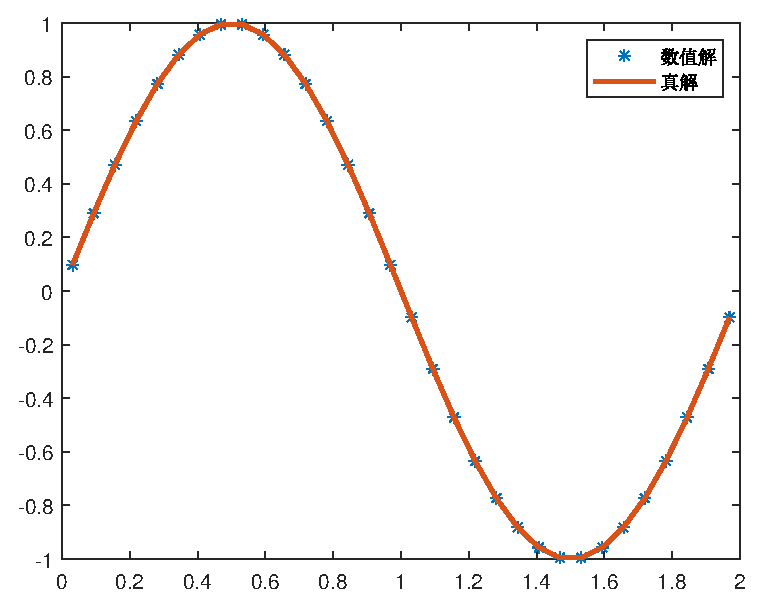
\includegraphics[width=0.3\linewidth]{fig/example1-t=0.0.eps}
    }\quad
    \subfloat[$t=0.2s$]{
        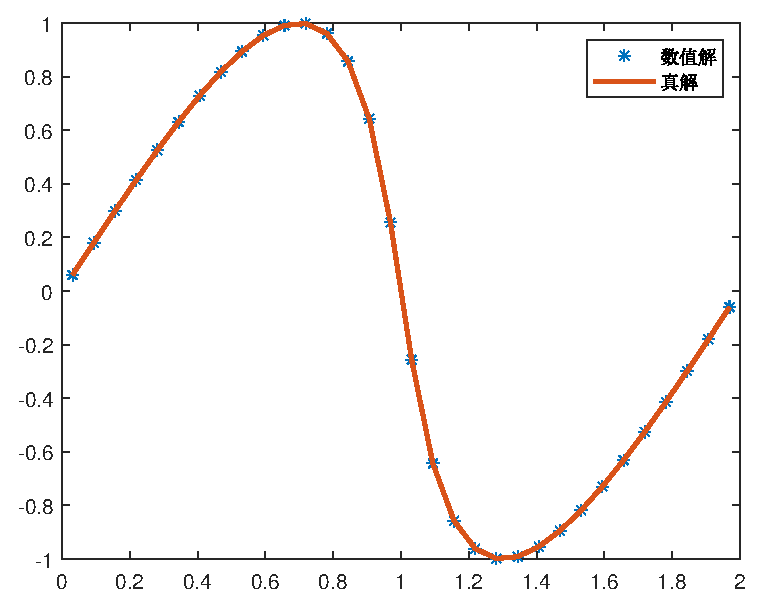
\includegraphics[width=0.3\linewidth]{fig/example1-t=0.2.eps}
    }\\
    \subfloat[$t=0.4s$]{
        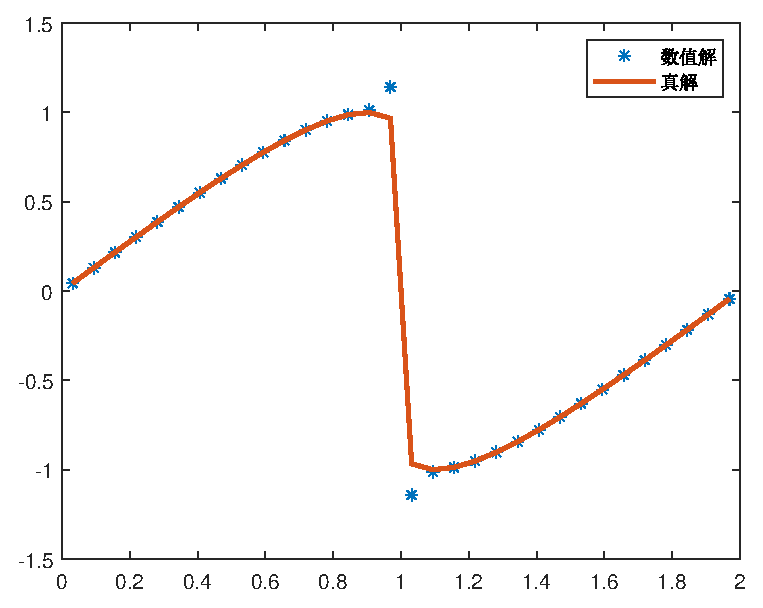
\includegraphics[width=0.3\linewidth]{fig/example1-t=0.4.eps}
    }\quad
    \subfloat[$t=0.6s$]{
        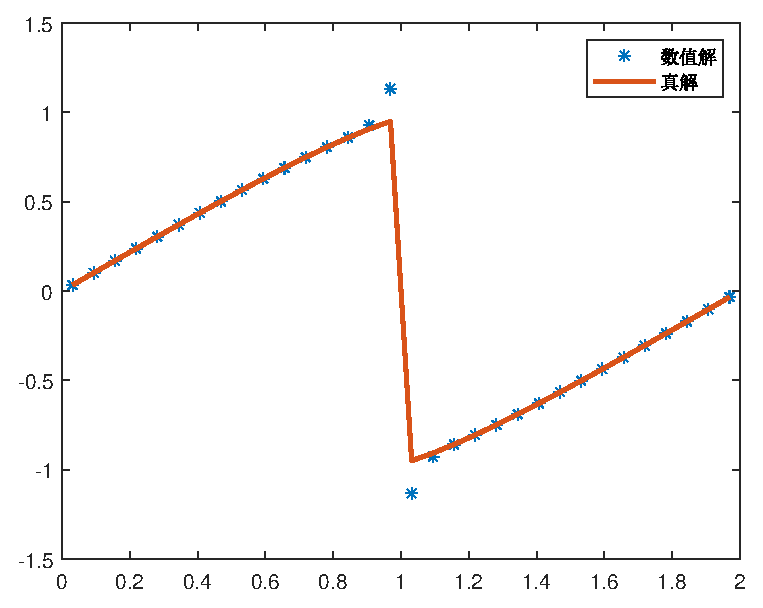
\includegraphics[width=0.3\linewidth]{fig/example1-t=0.6.eps}
    }\\
    \caption{上图为burgers方程在初值条件为$u=\sin(x)$时的演变}
    \label{间断示例}
\end{figure}


本文使用的数值方法为间断有限元(DG)法。让我们先简要回顾一下DG方法的历史。1973年,Reed和Hill\cite{Reed_Hill}在中子传输框架下提出了第一个不连续Galerkin(DG)方法。然后,Cockburn等人在一系列论文中 \cite{RKDG2,RKDG3,RKDG4,RKDG5} 对DG方法进行了重大发展,其中他们建立了一个框架,使用显式、非线性稳定的高阶Runge-Kutta时间离散化和DG空间离散化,使用精确或近似的Riemann解算器作为界面通量和总变差有界(TVB)限制器\cite{TVB},以实现对强不连续性的本质非振荡性。从那时起,这些方案被称为RKDG方法。但是,即使初始条件足够平滑,解决\eqref{equ:双曲守恒}也不容易,因为解可能包含强不连续性。不连续Galerkin(DG)方法可以捕捉弱不连续性而无需进一步修改。然而,对于存在强不连续性的问题,数值解可能在强震荡或接触不连续性附近具有显著的虚假震荡,特别是对于高阶数值方法而言。控制这些虚假震荡的常见策略是应用非线性限制器。

通常,使用限制器的过程可以分为两个步骤。首先,需要确定“坏单元”(也称为“有问题的单元”),即包含间断的单元,这些单元需要进行限制。其次,需要在这些“坏单元”中修正DG多项式解。由于守恒的要求,需要保证单元平均值不变,并且减小振荡。

在第一部分中,我们通常使用“坏单元”或称为间断指示器,这些指示器包括基于最小模型的指示器\cite{RKDG2}、基于力矩的指示器\cite{基于力矩的指示器}、改进的力矩指示器\cite{改进的基于矩的限制器}、以及基于DG超收敛性质的KXRCF指示器\cite{基于DG超收敛性质的KXRCF指示器}.

在第二部分中,一种限制器属于斜率型限制器,例如minmod类型限制器\cite{RKDG2,RKDG3,RKDG4,RKDG5},基于矩的限制器\cite{基于矩的限制器}和改进的基于矩的限制器\cite{改进的基于矩的限制器}等。它们的优点是可以在强间断附近有效抑制伪振荡的出现,但付出的代价是在解的光滑极值点处有可能降低格式的数值精度。另一种限制器基于加权本质非振荡(WENO)方法\cite{WENO1,WENO2,WENO3,WENO4,WENO5},它可以在平滑区域中实现高阶精度,并在强不连续性附近保持本质非振荡性质。WENO 格式一经提出,便引起人们的广泛关注,近二十年来,WENO 的各种变形格式层出不穷。例如:经典的WENO限制器(WENO-js)\cite{WENO-js1,WENO-js2},Hermite WENO限制器(HWENO)\cite{HWENO1,HWENO2},中心型 WENO 限制器(CWENO)\cite{CWENO},WENO-M限制器\cite{WENO-M},WENO-Z限制器\cite{WENO-Z}。但另一方面,基于WENO的限制器需要更广泛的空间模板来获得高阶方案。因此,在多维问题中,特别是在非结构化网格上,如三角形网格或四面体网格中实现它们是困难的。

\section{符号说明}
\begin{equation}
    \Delta_{+} w_{j}=w_{j+1}-w_{j}, \quad \Delta_{-} w_{j}=w_{j}-w_{j-1}
\end{equation}

\section{一维标量}
离散格式推导与稳定性证明见\cite{RN16}
\subsection{控制方程}
\begin{equation}
    u_t+f(u)_x = 0
\end{equation}
\subsection{空间离散格式}
\begin{equation}
    u_{h}(x, t)=\sum_{l=0}^{k} u_{i}^{(l)}(t) v_{l}^{(i)}(x), \quad x \in I_{i}
\end{equation}
其中 $u_i^{(l)}(t)$ 为自由度(degrees of freedom:dof)或矩,$v_l^{(i)}(x)$ 为基函数。当基函数为正交函数时,$u_i{(l)}(t)$ 的定义为:
\begin{equation}
    u_{i}^{(l)}(t)=\frac{1}{a_{l}} \int_{I_{i}} u_{h}(x, t) v_{l}^{(i)}(x) d x \quad l=0,1, \ldots, k
\end{equation}
其中 $a_{l}=\int_{I_{i}}\left(v_{l}^{(i)}(x)\right)^{2} d x$
\begin{remark}
    如果基函数不是正交函数,需要先求出质量矩阵的值,再求其逆矩阵。
\end{remark}

\begin{equation}
    \left\|v_{l}^{(j)}(x)\right\|^{2} \dfrac{\dd}{\dd t} u(t)+\left[\Delta_{-}\left(v_{l}^{(j)}\left(x_{j+1 / 2}\right) f_{j+1 / 2}\right)\right]-\int_{I_{j}} f\left(u^{h}(x, t)\right) \dfrac{\dd}{\dd x} v(x) \dd x=0
\end{equation}
数值通量:

满足三原则:
\begin{itemize}
    \item 一致性:$\widehat{f}(u, u)=f(u)$。
    \item 连续性:$\widehat{f}\left(u^{-}, u^{+}\right)$ 至少关于两个参数 $u^{-}$ 和 $u^{+}$ 是 Lipschitz 连续的。
    \item 单调性:$\widehat{f}\left(u^{-}, u^{+}\right)$ 是第一个参数 $u^{-}$ 的非降函数和第二个参数 $u^{+}$ 的非增函数。符号上,$\widehat{f}(\uparrow, \downarrow)$.
\end{itemize}
以下是几个常见的数值通量\cite{RN16}
\begin{itemize}
    \item Lax-Friedrichs flux
          \begin{equation}
              \widehat{f}^{L F}\left(u^{-}, u^{+}\right)=\frac{1}{2}\left(f\left(u^{-}\right)+f\left(u^{+}\right)-\alpha\left(u^{+}-u^{-}\right)\right), \quad \alpha=\max _{u}\left|f^{\prime}(u)\right|
          \end{equation}
    \item Local Lax-Friedrichs:
          \begin{equation}
              h^{\mathrm{LLF}}(a, b)=\frac{1}{2}[f(a)+f(b)-\beta(b-a)], \quad \beta=\max _{\min (a, b) \leq u \leq \max (a, b)}\left|f^{\prime}(u)\right|
          \end{equation}
          For convex  $f, f^{\prime \prime} \geq 0$ , one has  $\beta=\max \left(\left|f^{\prime}(a)\right|,\left|f^{\prime}(b)\right|\right) $
    \item Godunov flux
          \begin{equation}
              \widehat{f}^{G o d}\left(u^{-}, u^{+}\right)=\left\{\begin{array}{ll}
                  \min _{u^{-} \leq u \leq u^{+}} f(u), & \text { if } u^{-}<u^{+},     \\
                  \max _{u^{+} \leq u \leq u^{-}} f(u), & \text { if } u^{-} \geq u^{+}
              \end{array}\right.
          \end{equation}
    \item Engquist-Osher flux
          \begin{equation}
              \widehat{f}^{E O}=\int_{0}^{u^{-}} \max \left(f^{\prime}(u), 0\right) d u+\int_{0}^{u^{+}} \min \left(f^{\prime}(u), 0\right) d u+f(0)
          \end{equation}
\end{itemize}


\section{一维向量}

\begin{equation}
    \mathbf{U}_{t}+\mathbf{F}(\mathbf{U})_{x}=\mathbf{0}
\end{equation}

数值通量为:

\section{二维向量}
\subsection{控制方程}
\begin{equation}
    \partial_{t} \boldsymbol{u}+\operatorname{div} \boldsymbol{f} (\boldsymbol{u})=0
\end{equation}
\subsection{空间离散格式}
在每个小区间上做二维积分:
\begin{equation}
    \frac{d}{d t} \int_{K} u_{h}(t, x) v_{h}(x) d x+\int_{K} \operatorname{div} \mathbf{f}\left(u_{h}(t, x)\right) v_{h}(x) d x=0, \forall v_{h} \in V_{h}
\end{equation}
\begin{equation}
    \dfrac{\dd}{\dd t} \int_{K} u(x, t) v(x) \dd x+\sum_{e \in \partial K} \int_{e} \mathbf{f}(u(x, t)) \cdot n_{e, K} v(x) \dd \Gamma-\int_{K} \mathbf{f}(u(x, t)) \cdot \operatorname{grad} v(x) \dd x=0
\end{equation}
\begin{remark}
    特别的,对于矩形网格,有:
\end{remark}
其中 $n_{e,K}$ 是边界 $e$ 的标准外法向量。由于函数在小区间边界上间断 $f(u)$ 在 $e$ 上没有定义,和一维的情况类似,需要使用数值通量$h_{e, K}\left(u_{h}\left(t, x^{\operatorname{int}(K)}\right), u_{h}\left(t, x^{\operatorname{ext}(K)}\right)\right)$代替$\mathbf{f}\left(u_{h}(t, x)\right) \cdot \mathbf{n}_{e, K}$, 其中:
\begin{equation}
    \begin{array}{l}
        u_{h}\left(t, x^{i n t(K)}\right)= \lim _{\substack{y \rightarrow x \\
        y \in K}} u_{h}(t, y),                                              \\
        u_{h}\left(t, x^{e x t(K)}\right)=\left\{\begin{array}{ll}
                                                     \gamma_{h}(x, t),           & \text { if } x \in \partial \Omega, \\
                                                     \lim _{\substack{y \rightarrow x                                  \\
                                                     y \in(K)^{c}}} u_{h}(t, y), & \text { otherwise. }
                                                 \end{array}\right.
    \end{array}
\end{equation}

% \begin{equation}
%     \int_{e} \mathbf{f}(u(x, t)) \cdot n_{e, K} v_{h}(x) d \Gamma \approx \sum_{l=1}^{L} \omega_{l} \mathbf{f}\left(u\left(x_{e l}, t\right)\right) \cdot n_{e, K} v\left(x_{e l}\right)|e|,
% \end{equation}
% \begin{equation}
%     \int_{K} \mathbf{f}(u(x, t)) \cdot \operatorname{grad} v(x) d x \approx \sum_{j=1}^{M} \underline{\omega}_{j} \mathbf{f}\left(u\left(x_{K j}, t\right)\right) \cdot \operatorname{grad} v\left(x_{K j}\right)|K| .
% \end{equation}

\begin{equation}
    h_{e, K}(a, b)=\frac{1}{2}\left[\mathbf{f}(a) \cdot n_{e, K}+\mathbf{f}(b) \cdot n_{e, K}-\alpha_{e, K}(b-a)\right] .
\end{equation}
\section{指示子}
指示子英文为indicator。限制器的一个重要组成部分是指示子,指示子可以找出存在强间断的小区间。
\subsection{TVB指示子}
1、基于 minmod 函数的 TVB 限制器  [6]  (简称 TVB)
\begin{equation}
    u_{i+\frac{1}{2}}^{-}=u_{i}^{(0)}+\tilde{u}_{i}, \quad u_{i-\frac{1}{2}}^{+}=u_{i}^{(0)}-\tilde{\tilde{u}}_{i}
\end{equation}
我们可以看到

\begin{equation}
    \tilde{u}_{i}=\sum_{l=1}^{k} u_{i}^{(l)} v_{l}^{(i)}\left(x_{i+\frac{1}{2}}\right), \quad \tilde{\tilde{u}}_{i}=-\sum_{l=1}^{k} u_{i}^{(l)} v_{l}^{(i)}\left(x_{i-\frac{1}{2}}\right)
\end{equation}
\begin{equation}
    \tilde{u}_{j}^{(\mathrm{mod})}=m\left(\tilde{u}_{j}, \Delta_{+} u_{j}^{(0)}, \Delta_{-} u_{j}^{(0)}\right), \quad \tilde{\tilde{u}}^{(\bmod )}=m\left(\tilde{\tilde{u}}_{j}, \Delta_{+} u_{j}^{(0)}, \Delta_{-} u_{j}^{(0)}\right),
\end{equation}
其中
\begin{equation}
    m\left(a_{1}, a_{2}, \ldots, a_{n}\right)=\begin{cases}
        a_{1}                                             & \text { if }\left|a_{1}\right| \leq M h^{2}                                                                                              \\
        s \cdot \min _{1 \leq j \leq n}\left|a_{j}\right| & \text { if } \operatorname{sign}\left(a_{1}\right)=\operatorname{sign}\left(a_{2}\right)=\cdots=\operatorname{sign}\left(a_{n}\right)=s, \\
        0                                                 & \text { otherwise }
    \end{cases}
\end{equation}



\subsection{KXRCF指示子}
KXRCF指示子利用了DG方法的超收敛性\cite{RN92},把小单元 $I_{i,j}$ 的边界 $\partial I_{i,j}$ 分成 $\partial I_{i,j}^-,\partial I_{i,j}^+$ 两部分,分别对应流体流入和流出 $I_{i,j}$ 的边界。
\begin{equation}
    \frac{\left|\int_{\partial I_{i, j}^{-}}\left(\left.u_{h}(x, y, t)\right|_{I_{i, j}}-\left.u_{h}(x, y, t)\right|_{I_{l}}\right) d s\right|}{h_{i, j}^{R}\left|\partial I_{i, j}^{-}\right| \cdot||\mid \widehat{u_{h}}(x, y, t)|_{\partial I_{i, j}}\mid||} \geq C_{k},
\end{equation}
其中,$R=1$ 当 $k=1$, $R=1.5$ 当 $k>1$. $h_{i,j}$ 为 $I_{i,j}$ 外接圆的半径。$C_k$ 为常数,一般可取 $C_k = 1$. $I_l$ 为 $I_{i,j}$ 在 $\partial I_{i,j}^-$ 一侧的相邻单元。$u_h$ 可取守恒量,或者由守恒量引申出的物理量,$||\mid \widehat{u_{h}}(x, y, t)|_{\partial I_{i, j}}\mid||$ 为 $\mid \widehat{u_{h}}(x, y, t)|_{\partial I_{i, j}}\mid$ 在 $\partial I_{i,j}$ 上的最大值。$|\partial I_{i,j}^-|$ 为 $\partial I_{i,j}^-$ 的长度。
\section{限制器}
\subsection{TVB限制器}

\subsection{WENO-JS限制器}
WENO 全称为 Weighted Essentially Non-Oscillatory。WENO 限制器的思想是:使用周围的小区间上守恒量的平均值来重构当前小区间的函数,再使用得到的新函数来修正原高阶自由度,从而达到修正限制的目的。下面我们简单介绍 WENO 限制器在一维标量方程上的使用方法,一维系统的情况请参阅\cite{WENO-js1}.

\begin{enumerate}[label={{\bf Step \arabic*}:}]
    \item 首先我们在 Gauss 或 Gauss-Lobatto 积分点处重构 $u$ 的点值。对于基于 $\mathbb{P}^{k}$ 的 DG(精度为 $(k+1)$ 阶),我们需要一个至少精确到 $\mathrm{O}\left(h^{2 k+2}\right)$ 的 Gauss 或 Gauss-Lobatto 积分规则,而 WENO 重构的精度必须至少为 $2 k+1$。为此,我们需要使用相邻的 $2 k+1$ 个单元 $I_{i-k}\cdots I_{i+k}$ 的单元平均值来重构 u 的点值。
          \begin{enumerate}[label={\bf Step 1.\arabic*.}]
              \item 我们确定 $k+1$ 个小的模板 $S_{j}$,其中 $j=0,1,\cdots,k$,使得 $I_{i}$ 属于每个模板。记 $S_{j}=\cup_{l=0}^{k} I_{i+j-l}$。我们用 $\mathcal{T}=\cup_{j=0}^{k} S_{j}$ 表示包含所有 $k+1$ 个小模板的大模板.在每个模板 $S_j, j=0,\ldots,k$ 构造一个 $k$ 次多项式重构 $p_j(x)$,使得每个模板 $S_j$ 中每个单元格中 $p_j(x)$ 的平均值与给定的 $u$ 的单元格平均值相符,即\begin{equation}
                        \frac{1}{\Delta x_{i+j-l}} \int_{I_{i+j-l}} p_{j}(x) dx =u_{i+j-l}^{(0)},\quad l=0,\ldots,k.
                    \end{equation}
                    在更大的模板 $\mathcal{T}$ 上,我们再重构一个 $2k$ 次多项式 $Q(x)$,使得
                    \begin{equation}
                        \frac{1}{\Delta x_{i+l}} \int_{I_{i+l}} Q(x) dx=u_{i+l}^{(0)},\quad l=-k,\ldots,k.
                    \end{equation}
                    关于 $p_j(x)$ 和 $Q(x)$ 的构造细节可以在文献\cite{WENO5}中找到。
              \item 我们找到组合系数,也称为线性权重,记为 $\gamma_{0},\ldots,\gamma_{k}$,满足
                    \begin{equation}
                        Q(x_G)=\sum_{j=0}^k\gamma_j p_j(x_G)
                    \end{equation}
                    其中 $x_G$ 是 Gauss 积分点。不同的积分点对应不同的线性权重。
              \item 我们计算每个权重组 $S_j$ 的平滑度指示器,表示 $p_j(x)$ 在目标单元 $I_i$ 中的平滑程度。平滑度指示器 $\beta_j$ 越小,函数 $p_j(x)$ 在目标单元中的平滑度就越高,我们使用以下平滑度指示器:
                    \begin{equation}
                        \beta_{j}=\sum_{l=1}^{k} \int_{I_{i}} \Delta x_{i}^{2 l-1}\left(\frac{\partial^{l}}{\partial x^{l}} p_{j}(x)\right)^{2} d x
                    \end{equation}
              \item 我们基于平滑度指示器计算非线性权重,
                    \begin{equation}
                        \omega_{j}=\frac{\bar{\omega}_{j}}{\sum_{l} \bar{\omega}_{l}}, \quad \bar{\omega}_{j}=\frac{\gamma_{j}}{\sum_{j}\left(\varepsilon+\beta_{j}\right)^{2}},
                    \end{equation}
                    其中,$\gamma_j$ 是在 {\bf Step 1.2.} 中确定的线性权重,$\varepsilon$ 是一个很小的数,用于避免分母为零。在本文中,我们在所有计算中使用 $\varepsilon=10^{-6}$。最终的 WENO 近似为:
                    \begin{equation}
                        u_{(x_G)} \approx \sum_{j=0}^{k} \omega_{j} p_{j}\left(x_{G}\right)
                    \end{equation}
          \end{enumerate}
    \item 基于在 Gauss 积分点 $x_G$ 上重构的点值 $u(x_G)$ 和数值积分,我们得到重构函数的高阶自由度:
          \begin{equation}
              u_{i}^{(l)}=\frac{1}{||v_{l}^{(j)}||^2} \sum_{G} w_{G} u\left(x_{G}\right) v_{l}^{(i)}\left(x_{G}\right), \quad l=1, \ldots, k
          \end{equation}
          其中,$w_{G}$ 是 Gauss 积分点 $x_{G}$ 对应的高斯积分权重。
\end{enumerate}
\subsection{WENO-M}
\begin{equation}
    g_{k}(\omega)=\frac{\omega\left(\bar{\omega}_{k}+\bar{\omega}_{k}^{2}-3 \bar{\omega}_{k} \omega+\omega^{2}\right)}{\bar{\omega}_{k}^{2}+\omega\left(1-2 \bar{\omega}_{k}\right)}
\end{equation}
\begin{equation}
    \alpha_{k}^{*}=g_{k}\left(\omega_{k}^{(\mathrm{JS})}\right)
\end{equation}
\begin{equation}
    \omega_{k}^{(\mathrm{M})}=\frac{\alpha_{k}^{*}}{\sum_{i=0}^{2} \alpha_{i}^{*}}
\end{equation}

\subsection{WENO-Z}
\begin{equation}
    \tau_{5}=\left|\beta_{0}-\beta_{2}\right|
\end{equation}
\begin{equation}
    \beta_{k}^{z}=\left(\frac{\beta_{k}+\epsilon}{\beta_{k}+\tau_{5}+\epsilon}\right), \quad k=0,1,2
\end{equation}
\begin{equation}
    \omega_{k}^{z}=\frac{\alpha_{k}^{z}}{\sum_{l=0}^{2} \alpha_{l}^{z}}, \quad \alpha_{k}^{z}=\frac{d_{k}}{\beta_{k}^{z}}=d_{k}\left(1+\frac{\tau_{5}}{\beta_{k}+\epsilon}\right), \quad k=0,1,2
\end{equation}



\subsection{MR-WENO限制器}
\begin{enumerate}[label={{\bf Step \arabic*}:}]
    \item 1
          \begin{enumerate}[label={\bf Step 1.\arabic*.}]
              \item 在有问题的单元 $I_j$ 上定义一系列不同次数的多项式。我们构造多项式 $q_{\ell}(x), \ell=0, \ldots, k$,满足以下条件:
                    \begin{equation}
                        \int_{I_j} q_{\ell}(x) v_{l}^{j}(x) \dd x=\int_{I_j} u_{h}(x) v_{l}^{j}(x, y) \dd x,\, l=0,1, \ldots, \ell.
                    \end{equation}
                    \begin{remark}
                        如果我们采用规范正交基 $v_{l}^{(0)}(x)$,那么不同的多项式 $q_{\ell}(x), \ell=0,1,, \ldots, k$ 的构造非常简单。在这种情况下,我们可以直接得到多项式
                        \begin{equation}
                            q_{\ell}(x)=\sum_{l=0}^{\ell} u_{j}^{(l)}(t) v_{l}^{(j)}(x),\,\ell=0,1,\ldots, k.
                        \end{equation}
                    \end{remark}
              \item 我们通过以下方式构造多项式 $p_{\ell, \ell}(x),p_{\ell,\ell+1} \ell(x)=1, \ldots, k$
                    \begin{equation}
                        p_{\ell, \ell}(x)=\frac{1}{\gamma_{\ell, \ell}} q_{\ell}(x)-\frac{\gamma_{\ell-1, \ell}}{\gamma_{\ell, \ell}} p_{\ell-1, \ell}(x), \ell=1, \ldots, k,
                    \end{equation}
                    \begin{equation}
                        p_{\ell, \ell+1}(x)=\omega_{\ell, \ell} p_{\ell, \ell}(x)+\omega_{\ell-1, \ell} p_{\ell-1, \ell}(x), \ell=1, \ldots, k-1
                    \end{equation}
                    这些表达式中,$\gamma_{\ell-1, \ell}$ 和 $\gamma_{\ell, \ell}$ 是线性权重,要求 $\gamma_{\ell-1, \ell}+\gamma_{\ell, \ell}=1$,且 $\gamma_{\ell-1, \ell},\gamma_{\ell, \ell}>0$.由于对于平滑解来说,高阶解通常是最好的,因此我们给予高阶多项式更高的线性权重,基于低阶多项式更小的线性权重。即:
                    \begin{equation}
                        \gamma_{\ell_,\ell} \gg \gamma_{\ell-1,\ell}
                    \end{equation}
                    当比值 $\frac{\gamma_{\ell_,\ell}}{\gamma_{\ell-1,\ell}}$ 的值较小时,可以在不连续性上获得更好的结果,而当值较大时,通常对于平滑解更好。在我们的数值测试中,我们取
                    \begin{equation}
                        \gamma_{\ell-1, \ell}=0.01,\quad  \gamma_{\ell, \ell}=0.99,\quad \ell=1, \ldots, k
                    \end{equation}
                    这可以在平滑区域中保持原始的高阶,在所有数值例子中都可以保持基本上非振荡的冲击过渡。

                    $\omega_{\ell-1, \ell}$ 和 $\omega_{\ell, \ell}$ 是非线性权重(稍后将准确地介绍)。
              \item 计算光滑指示器  $\beta_{\ell, \ell_{2}}$ , 其衡量了  $p_{\ell, \ell_{2}}(x, y)$  for  $\ell=\ell_{2}-1 ,  \ell_{2} ; \ell_{2}=1,2,3,4$  在小区间  $I_{j}$ 上的光滑程度. 具体来说:$\beta_{\ell, \ell_{2}}$ 越小,说明 $p_{\ell, \ell_{2}}(x, y)$ 在 $I_{j}$ 上越光滑。
                    \begin{equation}
                        \label{eqa:光滑指示器}
                        \beta_{l_1,l_2}=\sum_{l=1}^{k} \int_{I_{i}} \Delta x_{i}^{2 l-1}\left(\frac{\partial^{l}}{\partial x^{l}} p_{l_1,l_2}(x)\right)^{2} d x
                    \end{equation}
                    由于 $p_{0,1}(x)$ 是一个常值函数,$p'_{0,1}(x)=0$,因此无法使用统一的\eqref{eqa:光滑指示器}式来衡量其光滑程度,因此我们为 $p_{0,1}(x)$ 设计了其独有的限制器:

                    定义线性函数 $q_{0,1}(x),q_{0,2}(x)$ 满足:

                    \begin{equation}
                        \begin{aligned}
                            \int_{I_{j-1}}q_{0,1}(x)v_{l}^{(j-1)}(x)\dd x & = \int_{I_{j-1}}u_h(x)v_{l}^{(j-1)}\dd x,\quad l=0,1,\cdots,k \\
                            \int_{I_{j+1}}q_{0,1}(x)v_{l}^{(j+1)}(x)\dd x & = \int_{I_{j+1}}u_h(x)v_{l}^{(j+1)}\dd x,\quad l=0,1,\cdots,k \\
                        \end{aligned}
                    \end{equation}
                    再构造 $\varsigma_1,\varsigma_2$,其定义如下:
                    \begin{equation}
                        \varsigma_1=\int_{I_{j}}\left(\frac{\dd}{\dd x}q_{0,1}\right)^2\dd x,\quad \varsigma_2=\int_{I_{j}}\left(\frac{\dd}{\dd x}q_{0,1}\right)^2\dd x\\
                    \end{equation}
                    $\beta_{0,1}$ 定义取 $\varsigma_1,\varsigma_2$ 的最小值:
                    \begin{equation}
                        \beta_{0,1} = \min\{\varsigma_1,\varsigma_2 \}.
                    \end{equation}
              \item    基于线性权重和光滑性指标计算非线性权重。我们采用文献\cite{WENO-Z} 中所示的WENO-Z的做法,$\tau_{\ell_{2}}$ 定义如下:
                    \begin{equation}
                        \tau_{\ell_2} = (\beta_{\ell_2,\ell_2}-\beta_{\ell_2-1,\ell_2})^2
                    \end{equation}
                    \begin{equation}
                        \omega_{\ell_{1}, \ell_{2}}=\frac{\bar{\omega}_{\ell_{1}, \ell_{2}}}{\sum_{\ell=\ell_{2}-1}^{\ell_{2}} \bar{\omega}_{\ell, \ell_{2}}},\quad \bar{\omega}_{\ell_{1}, \ell_{2}}=\gamma_{\ell_{1},\ell_{2}}\left(1+\frac{\tau_{\ell_2}}{\epsilon+\beta_{\ell_1,\ell_2}}\right)
                    \end{equation}
                    得到最终的拟合函数:
                    \begin{equation}
                        p^{\text {new }}(x)=\sum_{\ell=\ell_{2}-1}^{\ell_{2}} \omega_{\ell, \ell_{2}} p_{\ell, \ell_{2}}(x), \quad \ell_{2}=1,2,3,4,
                    \end{equation}
                    \begin{equation}
                        u_{j}^{(l)}(t)=\frac{1}{||v_{l}^{(j)}||^{2}} \int_{I_{j}} u(x, t) v_{l}^{(j)}(x) d x, \quad l=0,1,\cdots, k .
                    \end{equation}
          \end{enumerate}
    \item 修正高阶矩
\end{enumerate}


\begin{remark}
    如果不修正线性权重,那么最终会得到 $p^{\text {new }}(x)=p^{\text {old }}(x)$.
    \begin{equation}
        \begin{aligned}
            p^{\text {new }}(x) & =\gamma_{l_1,l_2}p_{l_1,l_2}(x)+\gamma_{l_2,l_2}p_{l_2,l_2}(x)                                                                                            \\
                                & =\gamma_{l_1,l_2}p_{l_1,l_2}(x)+\gamma_{l_2,l_2}\left(\frac{1}{\gamma_{l_2,l_2}}q_{l_2}(x)-\frac{\gamma_{l_1,l_2}}{\gamma_{l_2,l_2}}p_{l_1,l_2}(x)\right) \\
                                & =q_{l_2}(x)=p^{\text {old }}(x)
        \end{aligned}
    \end{equation}
\end{remark}

\begin{equation}
    \beta_{\ell, \ell_{2}}=\sum_{|\alpha|=1}^{\kappa} \int\left(\Delta x_{i} \Delta y_{j}\right)^{|\alpha|-1}\left(\frac{\partial^{|\alpha|}}{\partial x^{\alpha_{1}} \partial y^{\alpha_{2}}} p_{\ell, \ell_{2}}(x, y)\right)^{2} d x d y
\end{equation}


特别的:
\begin{equation}
    \begin{aligned}
        p_{01} & = q_0                                                             \\
        p_{11} & = \frac{1}{\gamma_{11}}q_1-\frac{\gamma_{01}}{\gamma_{11}}p_{01}  \\
        p_{12} & =\omega_{11}p_{11} + \omega_{01}p_{0,1}                           \\
        p_{22} & =\frac{1}{\gamma_{22}}q_2 - \frac{\gamma_{12}}{\gamma_{22}}p_{12} \\
    \end{aligned}
\end{equation}

\begin{equation}
    \begin{aligned}
        p^{\text {MR-WENO2 }}(x, y, z) & =\omega_{0,1} p_{0,1}(x, y, z)+\omega_{1,1} p_{1,1}(x, y, z),          \\
        p^{\text{MR-WENO3}}(x, y, z)   & =\omega_{1,2} p^{M R-W E N O 2}(x, y, z)+\omega_{2,2} p_{2,2}(x, y, z)
    \end{aligned}
\end{equation}

\section{保极值限制器}

\newpage
\begin{appendix}
    \section{边界条件}
    \subsection{周期性边界条件}
    \subsection{冯诺依曼边界条件}
    \section{数学符号}
    \subsection{散度}
    在三维直角坐标系  $x y z$  中,设向量场  $\boldsymbol{A}$  的表示为
    $\boldsymbol{A}(x, y, z)=A_{x}(x, y, z) \boldsymbol{i}+A_{y}(x, y, z) \boldsymbol{j}+A_{z}(x, y, z) \boldsymbol{k}$ 其中的  $\boldsymbol{i}, \boldsymbol{j}, \boldsymbol{k} $ 分别是  $x$  轴、  $y$  轴、  $z$  轴方向上的单位向量,场的分量  $A_{x}, A_{y}, A_{z}$  具有一阶连续偏导数,那么向量场  $\boldsymbol{A}$  的散度就是:
    \begin{equation}
        \operatorname{div} \boldsymbol{A}=\div \boldsymbol{A}=\dfrac{\partial A_{x}}{\partial x}+\dfrac{\partial A_{y}}{\partial y}+\dfrac{\partial A_{z}}{\partial z}
    \end{equation}
    \subsection{梯度}
    $\nabla f$在三维直角坐标系中表示为
    \begin{equation}
        {\displaystyle \nabla f={\begin{pmatrix}{\dfrac {\partial f}{\partial x}},{\dfrac {\partial f}{\partial y}},{\dfrac {\partial f}{\partial z}}\end{pmatrix}}={\dfrac {\partial f}{\partial x}}\mathbf {i} +{\dfrac {\partial f}{\partial y}}\mathbf {j} +{\dfrac {\partial f}{\partial z}}\mathbf {k} }
    \end{equation}
    $i, j, k $为标准的单位向量,分别指向 $x, y$ 跟 $z$ 坐标的方向。
    \subsection{范数}
    范数(norm)是一个函数,它将一个向量映射到非负实数。在机器学习和优化中,范数是一种衡量向量大小或长度的方式。

    L1, L2和L无穷范数是线性代数中的三种不同的向量范数(或向量长度度量),它们在数学和数据科学领域中经常使用。

    L1范数:L1范数也称为曼哈顿距离,它是一个向量中每个元素的绝对值之和。对于一个$n$维向量$x = (x1, x2, ..., xn)$,其$L1$范数定义如下:
    \begin{equation}
        ||x||_1 = |x_1| + |x_2| + \cdots + |x_n|
    \end{equation}

    L2范数:L2范数也称为欧几里得距离,它是向量中每个元素平方和的平方根。对于一个$n$维向量$x = (x_1, x_2,\cdots, x_n)$,其L2范数定义如下:
    \begin{equation}
        ||x||_2 = \sqrt{(x_1^2 + x_2^2 + ... + x_n^2)}
    \end{equation}
    $L_\infty$范数:$L_\infty$ 范数也称为最大值范数,它是向量中所有元素的绝对值中最大的值。对于一个n维向量$x = (x_1, x_2,\cdots, x_n)$,其$L_\infty$定义如下:
    \begin{equation}
        ||x||_\infty = \max(|x_1|, |x_2|,\cdots, |x_n|)
    \end{equation}
    这些向量范数在机器学习和优化算法中经常使用,例如L1和L2正则化(用于缩小模型参数),L1和L2距离度量(用于计算相似性或距离),以及L1和L2约束(用于限制变量的取值范围)。
    \newpage
    \section{控制方程}
    \subsection{一维方程}
    \subsubsection{欧拉方程}
    \paragraph{方程形式}
    \begin{equation}
        \mathbf{U}=\left[\begin{array}{l}
                u_{1} \\
                u_{2} \\
                u_{3}
            \end{array}\right] \equiv\left[\begin{array}{c}
                \rho   \\
                \rho u \\
                E
            \end{array}\right], \quad \mathbf{F}=\left[\begin{array}{c}
                f_{1} \\
                f_{2} \\
                f_{3}
            \end{array}\right] \equiv\left[\begin{array}{c}
                \rho u       \\
                \rho u^{2}+p \\
                u(E+p)
            \end{array}\right]
    \end{equation}
    或
    \begin{equation}
        \mathbf{F}(\mathbf{U})=\left[\begin{array}{l}
                f_{1} \\
                f_{2} \\
                f_{3}
            \end{array}\right] \equiv\left[\begin{array}{c}
                u_{2}                                                            \\
                \dfrac{1}{2}(3-\gamma) \dfrac{u_{2}^{2}}{u_{1}}+(\gamma-1) u_{3} \\
                \gamma \dfrac{u_{2}}{u_{1}} u_{3}-\dfrac{1}{2}(\gamma-1) \dfrac{u_{2}^{3}}{u_{1}^{2}}
            \end{array}\right]
    \end{equation}
    这里 $\rho$ 为密度,$p$为压力,$u$为粒子速度,$E$ 为每单位体积的总能量。
    \begin{equation}
        E=\dfrac{1}{2}\rho u^{2}+\frac{p}{\gamma-1}
    \end{equation}

    对于空气,一般可取 $\gamma=1.4$.声速 $a$ 的表达式为:
    \begin{equation}
        a=\sqrt{\left(p / \rho^{2}-e_{\rho}\right) / e_{p}}=\sqrt{\dfrac{\gamma p}{\rho}}
    \end{equation}

    \paragraph{特征分析}
    Jacobian 矩阵为:
    \begin{equation}
        \mathbf{A}(\mathbf{U})=\dfrac{\partial \mathbf{F}}{\partial \mathbf{U}}=\left[\begin{array}{l}
                \partial f_{1} / \partial u_{1} \partial f_{1} / \partial u_{2} \partial f_{1} / \partial u_{3} \\
                \partial f_{2} / \partial u_{1} \partial f_{2} / \partial u_{2} \partial f_{2} / \partial u_{3} \\
                \partial f_{3} / \partial u_{1} \partial f_{3} / \partial u_{2} \partial f_{3} / \partial u_{3}
            \end{array}\right]
    \end{equation}

    \begin{equation}
        \mathbf{A}(\mathbf{U})=\begin{bmatrix}
            0                                                                                      & 1                                                                                       & 0                                       \\
            -\dfrac{1}{2}(\gamma-3)\left(\dfrac{u_{2}}{u_{1}}\right)^{2}                           & (3-\gamma)\left(\dfrac{u_{2}}{u_{1}}\right)                                             & \gamma-1                                \\
            -\dfrac{\gamma u_{2} u_{3}}{u_{1}^{2}}+(\gamma-1)\left(\dfrac{u_{2}}{u_{1}}\right)^{3} & \dfrac{\gamma u_{3}}{u_{1}}-\dfrac{3}{2}(\gamma-1)\left(\dfrac{u_{2}}{u_{1}}\right)^{2} & \gamma\left(\dfrac{u_{2}}{u_{1}}\right)
        \end{bmatrix}
    \end{equation}
    \begin{equation}
        \begin{bmatrix}
            0                                          & 1                                                   & 0          \\
            -\dfrac{1}{2}(3-\gamma) u^{2}              & (3-\gamma) u                                        & (\gamma-1) \\
            -\gamma \dfrac{E u}{\rho}+(\gamma-1) u^{3} & \gamma \dfrac{E}{\rho}-\dfrac{3}{2}(\gamma-1) u^{2} & \gamma u
        \end{bmatrix}
    \end{equation}

    $\mathbf{A}(\mathbf{U})$ 的特征值为:
    \begin{equation}
        \lambda_{1}=u-a, \lambda_{2}=u, \lambda_{3}=u+a
    \end{equation}
    左右特征向量为\cite{RN95}:
    \begin{equation}
        L_{j}(u)=\left(\begin{array}{ccc}
                \dfrac{B_{2}+\mu / c}{2} & -\dfrac{B_{1} \mu+1 / c}{2} & \dfrac{B_{1}}{2} \\
                1-B_{2}                  & B_{1} \mu                   & -B_{1}           \\
                \dfrac{B_{2}-\mu / c}{2} & -\dfrac{B_{1} \mu-1 / c}{2} & \dfrac{B_{1}}{2}
            \end{array}\right)
    \end{equation}
    \begin{equation}
        R_{j}(u)=\left(\begin{array}{ccc}
                1       & 1           & 1       \\
                \mu-c   & \mu         & \mu+c   \\
                H-c \mu & \mu^{2} / 2 & H+c \mu
            \end{array}\right)
    \end{equation}
    $\text { where } c=\sqrt{\gamma p / \rho}, B_{1}=(\gamma-1) / c^{2}, B_{2}=B_{1} \mu^{2} / 2 \text { and } H=(E+p) / \rho \text {. }$
    对应的右特征向量为:
    \begin{equation}
        \mathbf{K}^{(1)}=\left[\begin{array}{c}
                1   \\
                u-a \\
                H-u a
            \end{array}\right], \mathbf{K}^{(2)}=\left[\begin{array}{c}
                1 \\
                u \\
                \dfrac{1}{2} u^{2}
            \end{array}\right], \mathbf{K}^{(3)}=\left[\begin{array}{c}
                1   \\
                u+a \\
                H+u a
            \end{array}\right]
    \end{equation}
    其中 $H$ 为总比焓(total specific enthalpy),$h$ 为比焓(specific enthalpy).
    \begin{equation}
        H=(E+p) / \rho \equiv \dfrac{1}{2} u^{2}+h, \quad h=e+p / \rho
    \end{equation}
    \paragraph{算例}
    \begin{example}
        \begin{equation}
            \begin{aligned}
                \rho(x, 0) & =1+0.2 \sin \pi x \\
                u(x, 0)    & =0.7              \\
                p(x, 0)    & =1
            \end{aligned}
        \end{equation}
        计算区域为 $[0,2]$, 周期边界条件,解析解为:
        \begin{equation}
            \begin{aligned}
                \rho(x, t) & =1+0.2 \sin \pi(x-0.7 t) \\
                u(x, t)    & =0.7                     \\
                p(x, t)    & =1
            \end{aligned}
        \end{equation}


    \end{example}
    \begin{example}
        Lax 激波管问题\cite{RN109}:
        \begin{equation}
            \begin{aligned}
                (\rho, v, p) & =(0.445,0.698,3.528) & \text { 当 } x \leqslant 0 \text {, } \\
                (\rho, v, p) & =(0.5,0,0.571) \quad & \text { 当 } \quad x>0 \text {. }     \\
            \end{aligned}
        \end{equation}
        计算区域为 $[-5,5]$ 两瑞均是常数边界条件, 我们求解该问题至 $T=1.3$.
    \end{example}

    \begin{example}
        Shu Osher 问题\cite{RN109},
        \begin{equation}
            \begin{aligned}
                (\rho, v, p) & =(3.857143,2.629369,10.333333)   & \text { 当 } x \leq-4, \\
                (\rho, v, p) & =(1+\varepsilon \sin (5 x), 0,1) & \text { 当 } x>-4 .
            \end{aligned}
        \end{equation}
        选取 $\epsilon = 0.2$,计算区域为 $[-5,5]$,两端边界条件按初值条件给定后保持不变,求解至时间 $T=1.8$
    \end{example}

    \subsection{二维方程}
    \subsubsection{欧拉方程}
    \paragraph{方程形式}
    \begin{equation}
        \mathbf{U}_{t}+\mathbf{F}(\mathbf{U})_{x}+\mathbf{G}(\mathbf{U})_{y}=\mathbf{0}
    \end{equation}
    其中
    \begin{equation}
        \mathbf{U}=\left[\begin{array}{c}
                \rho   \\
                \rho u \\
                \rho v \\
                E
            \end{array}\right], \quad \mathbf{F}=\left[\begin{array}{c}
                \rho u       \\
                \rho u^{2}+p \\
                \rho u v     \\
                u(E+p)
            \end{array}\right], \quad \mathbf{G}=\left[\begin{array}{c}
                \rho v       \\
                \rho u v     \\
                \rho v^{2}+p \\
                v(E+p)
            \end{array}\right]
    \end{equation}
    其中
    \begin{equation}
        E=\dfrac{p}{\gamma-1}+\dfrac{1}{2} \rho\left(u^{2}+v^{2}\right)
    \end{equation}
    同时
    \begin{equation}
        F = \begin{bmatrix}
            u_2                                                                          \\
            \dfrac{u_2^2}{u_1}+(\gamma-1)u_4+\dfrac{1-\gamma}{2}\dfrac{u_2^2+u_3^2}{u_1} \\
            \dfrac{u_2u_3}{u_1}                                                          \\
            \dfrac{u_2}{u_1}\left(\gamma u_4+\dfrac{1-\gamma}{2}\dfrac{u_2^2+u_3^2}{u_1}\right)
        \end{bmatrix}
        ,\quad G=\begin{bmatrix}
            u_3                                                                          \\
            \dfrac{u_2u_3}{u_1}                                                          \\
            \dfrac{u_3^2}{u_1}+(\gamma-1)u_4+\dfrac{1-\gamma}{2}\dfrac{u_2^2+u_3^2}{u_1} \\
            \dfrac{u_3}{u_1}\left(\gamma u_4+\dfrac{1-\gamma}{2}\dfrac{u_2^2+u_3^2}{u_1}\right)
        \end{bmatrix}
    \end{equation}

    \paragraph{特征分析}
    特征值为
    \begin{equation}
        \lambda_{1}=u-a, \quad \lambda_{2}=\lambda_{3}=u, \quad \lambda_{4}=u+a
    \end{equation}

    \begin{equation}
        \begin{bmatrix}
            0                                                                                                & 1                                                                                                   & 0                                         & 0                           \\
            \dfrac{\gamma (u_{2}-3)^{2}+(\gamma-1) u_{3}^{2}}{2 u_{1}^{2}}                                   & -(\gamma-3)\dfrac{u_{2}}{u_{1}}                                                                     & -(\gamma-1)\dfrac{u_{3}}{u_{1}}           & \gamma-1                    \\
            -\dfrac{u_{2} u_{3}}{u_{1}^{2}}                                                                  & \dfrac{u_{3}}{u_{1}}                                                                                & \dfrac{u_{2}}{u_{1}}                      & 0                           \\
            \dfrac{u_{2}}{u_1}\dfrac{\left((\gamma-1)(u_{2}^{2}+u_3^2)-\gamma u_{1} u_{4}\right)}{u_{1}^{2}} & \dfrac{3 u_{2}^{2}-\gamma u_{3}^{2}-3 \gamma u_{2}^{2}+u_{3}^{2}+2 \gamma u_{1} u_{4}}{2 u_{1}^{2}} & -\dfrac{u_{2} u_{3}(\gamma-1)}{u_{1}^{2}} & \dfrac{\gamma u_{2}}{u_{1}}
        \end{bmatrix}
    \end{equation}
    \begin{equation}
        \begin{bmatrix}
            0                                                                                             & 0                                                        & 1                                                                                       & 0                           \\
            -\dfrac{u_2 \,u_3 }{{u_1 }^2 }                                                                & \dfrac{u_3 }{u_1 }                                       & \dfrac{u_2 }{u_1 }                                                                      & 0                           \\
            \dfrac{\gamma \,{u_2 }^2 +\gamma \,{u_3 }^2 -{u_2 }^2 -3\,{u_3 }^2 }{2\,{u_1 }^2 }            & -\dfrac{u_2 \,{\left(\gamma -1\right)}}{u_1 }            & -\dfrac{u_3 \,{\left(\gamma -3\right)}}{u_1 }                                           & \gamma -1                   \\
            \dfrac{u_3}{u_1}\dfrac{{\left((\gamma-1)(u_2^2+u_3^2)-\gamma \,u_1 \,u_4 \right)}}{{u_1 }^2 } & -{\left(\gamma -1\right)}\dfrac{u_2 \,u_3 \,}{{u_1 }^2 } & \dfrac{(1-\gamma){u_2 }^2 +3(1-\gamma)\,{u_3 }^2 +2\,\gamma \,u_1 \,u_4 }{2\,{u_1 }^2 } & \dfrac{\gamma \,u_3 }{u_1 }
        \end{bmatrix}
    \end{equation}

    \begin{equation}
        F_U=\begin{bmatrix}
            0                                                     & 1                  & 0               & 0        \\
            -u^{2}+\dfrac{1}{2}(\gamma-1) \mathbf{V}^{2}          & (3-\gamma) u       & -(\gamma-1) v   & \gamma-1 \\
            -u v                                                  & v                  & u               & 0        \\
            u\left[\dfrac{1}{2}(\gamma-1) \mathbf{V}^{2}-H\right] & H-(\gamma-1) u^{2} & -(\gamma-1) u v & \gamma u
        \end{bmatrix} .
    \end{equation}
    其中 $\mathbf{V}^2=v^2+u^2$,

    左右特征向量为\cite{RN95}:
    \begin{equation}
        L_{i j}^{x}(u)=\begin{bmatrix}
            \dfrac{B_{2}+\mu / c}{2} & -\dfrac{B_{1} \mu+1 / c}{2} & -\dfrac{B_{1} v}{2} & \dfrac{B_{1}}{2} \\
            v                        & 0                           & -1                  & 0                \\
            1-B_{2}                  & B_{1} \mu                   & B_{1} v             & -B_{1}           \\
            \dfrac{B_{2}-\mu / c}{2} & -\dfrac{B_{1} \mu-1 / c}{2} & -\dfrac{B_{1} v}{2} & \dfrac{B_{1}}{2}
        \end{bmatrix},\quad
        R_{i j}^{x}(u)=\begin{bmatrix}
            1       & 0  & 1                        & 1       \\
            \mu-c   & 0  & \mu                      & \mu+c   \\
            v       & -1 & v                        & v       \\
            H-c \mu & -v & \dfrac{\mu^{2}+v^{2}}{2} & H+c \mu
        \end{bmatrix}
    \end{equation}

    \begin{equation}
        L_{i j}^{y}(u)=\begin{bmatrix}
            \dfrac{B_{2}+v / c}{2} & -\dfrac{B_{1} \mu}{2} & -\dfrac{B_{1} v+1 / c}{2} & \dfrac{B_{1}}{2} \\
            -\mu                   & 1                     & 0                         & 0                \\
            1-B_{2}                & B_{1} \mu             & B_{1} v                   & -B_{1}           \\
            \dfrac{B_{2}-v / c}{2} & -\dfrac{B_{1} \mu}{2} & -\dfrac{B_{1} v-1 / c}{2} & \dfrac{B_{1}}{2}
        \end{bmatrix},\quad
        R_{i j}^{y}(u)=\begin{bmatrix}
            1     & 0   & 1                        & 1     \\
            \mu   & 1   & \mu                      & \mu   \\
            v-c   & 0   & v                        & v+c   \\
            H-c v & \mu & \dfrac{\mu^{2}+v^{2}}{2} & H+c v
        \end{bmatrix}
    \end{equation}
    where  $c=\sqrt{\gamma p / \rho}, B_{1}=(\gamma-1) / c^{2}, B_{2}=B_{1}\left(\mu^{2}+v^{2}\right) / 2$  and  $H=(E+p) / \rho$
    \paragraph{算例}
    \begin{example}
        光滑问题:初值为:
        \begin{equation}
            \begin{aligned}
                \rho(x,y,0) & = 1+0.2\sin(\pi(x+y)) \\
                u(x,y,0)    & = 0.7                 \\
                v(x,y,0)    & = 0.3                 \\
                p(x,y,0)    & = 1                   \\
            \end{aligned}
        \end{equation}
        周期边界条件

        准确解为:
        \begin{equation}
            \rho(x,y,t) = 1+0.2\sin(\pi(x+y-(u+v)t)),u=0.7,v=0.3,p=1
        \end{equation}
    \end{example}
    \begin{example}
        二维黎曼问题\cite{RN13},初值为
        \begin{equation}
            \begin{cases}
                \left(\rho_{1}, p_{1}, \mu_{1}, v_{1}\right)^{T}=(0.5313,0.4,0,0)^{T}, & x>1, y>1, \\
                \left(\rho_{2}, p_{2}, \mu_{2}, v_{2}\right)^{T}=(1,1,0,0.7276)^{T},   & x>1, y<1, \\
                \left(\rho_{3}, p_{3}, \mu_{3}, v_{3}\right)^{T}=(1,1,0.7276,0)^{T},   & x<1, y>1, \\
                \left(\rho_{4}, p_{4}, \mu_{4}, v_{4}\right)^{T}=(0.8,1,0,0)^{T},      & x<1, y<1  \\
            \end{cases}
        \end{equation}
        $p_1<p_2=p_3=p_4$。滑移边界条件。建议计算至$t=0.52$,网格为260*260.


    \end{example}
    \newpage
    \section{基函数函数}
    \cite{RN48}
    \subsection{一维}
    在 $[-1,1]$ 上的勒让德函数为:
    \begin{equation}
        \begin{aligned}
            \varphi_{0}(\xi) & =1                                        \\
            \varphi_{1}(\xi) & =\xi                                      \\
            \varphi_{2}(\xi) & =\left(3 \xi^{2}-1\right) / 2             \\
            \varphi_{3}(\xi) & =\left(5 \xi^{3}-3 \xi\right) / 2         \\
            \varphi_{4}(\xi) & =\left(35 \xi^{4}-30 \xi^{2}+3\right) / 8
        \end{aligned}
    \end{equation}
    积分值为:
    \begin{equation}
        \int_{-1}^{-1}\varphi_i^2\dd x=\frac{2}{2n+1},n=0,1,2,\cdots
    \end{equation}

    \subsection{二维}
    \begin{equation}
        \begin{aligned}
            \varphi_{1}(\xi, \eta)  & =1                                                                             \\
            \varphi_{2}(\xi, \eta)  & =\xi                                                                           \\
            \varphi_{3}(\xi, \eta)  & =\eta                                                                          \\
            \varphi_{4}(\xi, \eta)  & =\dfrac{1}{2}\left(3 \xi^{2}-1\right)                                          \\
            \varphi_{5}(\xi, \eta)  & =\varphi_{2} \cdot \varphi_{3}=\xi \cdot \eta                                  \\
            \varphi_{6}(\xi, \eta)  & =\dfrac{1}{2}\left(3 \eta^{2}-1\right)                                         \\
            \varphi_{7}(\xi, \eta)  & =\left(5 \xi^{3}-3 \xi\right) / 2                                              \\
            \varphi_{8}(\xi, \eta)  & =\varphi_{4} \cdot \varphi_{3}=\dfrac{1}{2}\left(3 \xi^{2}-1\right) \cdot \eta \\
            \varphi_{9}(\xi, \eta)  & =\varphi_{6} \cdot \varphi_{2}=\dfrac{1}{2}\left(3 \eta^{2}-1\right) \cdot \xi \\
            \varphi_{10}(\xi, \eta) & =\left(5 \eta^{3}-3 \eta\right) / 2
        \end{aligned}
    \end{equation}
    \section{龙格库塔法}
    $\Delta t$ 的取值大小要求为:\cite{RN109}
    \begin{equation}
        \alpha \frac{\Delta t}{\Delta x} \leq \text{CFL}
    \end{equation}
    即:
    \begin{equation}
        \Delta t \leqslant \frac{\Delta x}{\alpha}\text{CFL}
    \end{equation}
    对于二维情况,
    \begin{equation}
        \Delta t \leqslant \frac{\Delta x}{\alpha}\text{CFL}
    \end{equation}

    \subsection{ssp 二阶龙格库塔法}
    ssp(strong stability-preserving)方法见:\cite{RN96}
    \begin{equation}
        \begin{aligned}
            u^{(1)} & =u^{n}+\Delta t L\left(u^{n}\right)                                               \\
            u^{n+1} & =\frac{1}{2} u^{n}+\frac{1}{2} u^{(1)}+\frac{1}{2} \Delta t L\left(u^{(1)}\right)
        \end{aligned}
    \end{equation}
    \subsection{ssp 三阶龙格库塔法}
    \begin{equation}
        \begin{aligned}
            u^{(1)} & =u^{n}+\Delta t L\left(u^{n}\right)                                                \\
            u^{(2)} & =\frac{3}{4} u^{n}+\frac{1}{4} u^{(1)}+\frac{1}{4} \Delta t L\left(u^{(1)}\right), \\
            u^{n+1} & =\frac{1}{3} u^{n}+\frac{2}{3} u^{(2)}+\frac{2}{3} \Delta t L\left(u^{(2)}\right),
        \end{aligned}
    \end{equation}
    \subsection{三阶龙格库塔法}
    \begin{equation}
        \begin{aligned}
            k_1     & = f(t_n, y_n)                                \\
            k_2     & = f(t_n + \frac{h}{2}, y_n + \frac{h}{2}k_1) \\
            k_3     & = f(t_n + h, y_n - hk_1 + 2hk_2)             \\
            y_{n+1} & = y_n + \frac{h}{6}(k_1 + 4k_2 + k_3)        \\
        \end{aligned}
    \end{equation}

    \subsection{四阶龙格库塔法}
    \begin{equation}
        \begin{aligned}
            k_{1}   & =f\left(t_{n}, y_{n}\right)                                \\
            k_{2}   & =f\left(t_{n}+\frac{h}{2}, y_{n}+\frac{h}{2} k_{1}\right)  \\
            k_{3}   & =f\left(t_{n}+\frac{h}{2}, y_{n}+\frac{h}{2} k_{2}\right)  \\
            k_{4}   & =f\left(t_{n}+h, y_{n}+h k_{3}\right)                      \\
            y_{n+1} & =y_{n}+\frac{h}{6}\left(k_{1}+2 k_{2}+2 k_{3}+k_{4}\right)
        \end{aligned}
    \end{equation}
    \section{数值积分}
    一般采用的求积公式是机械求解求积公式中的高斯积分。高斯积分是一种非常常用的数值积分方法,具有如下优点:
    \begin{itemize}
        \item 高斯积分的精度随着积分点的增加而增加,当积分点的数量足够大时,可以达到非常高的精度。
        \item 当使用的点数固定为 $n+1$ 个时,高斯积分具有 $2n+1$ 阶的精度,是所有机械求积公式中最高的。因此在计算复杂函数积分时,高斯积分可以显著减少计算时间和计算成本。
        \item 高斯积分公式可以非常方便地使用代码实现。
    \end{itemize}
    具体而言,该公式可写成:
    \begin{equation}
        \int_{-1}^1 f(x)\dd x=\sum_{i=1}^{n+1}\omega_if(x_i)
    \end{equation}
    其中,$\omega_i$ 和 $x_i$ 分别表示高斯积分公式中第 $i$ 个点的权重和位置。对于积分区间非 $[-1,1]$ 的积分,可以使用下面的公式:
    \begin{equation}
        \int_{a}^{b} f(x) \mathrm{d} x=\int_{-1}^{1} f\left(\frac{(b-a) t+b+a}{2}\right) \frac{b-a}{2} \mathrm{~d} t=\sum_i f(\frac{(b-a)x_i+b+a}{2})\frac{b-a}{2}\omega_i
    \end{equation}

    表 \ref{tab:高斯积分} 给出 $n=1,2,3,4,5$ 时,高斯积分的取值点和权重大小.
    \begin{table}[ht]
        \centering
        \caption{Gauss-Legendre的取值点和权重大小}
        \label{tab:高斯积分}
        \begin{tabular}{|c|c|c|}
            \hline
            $n$ & 取值点 $x_i$                                 & 权重 $w_i$                         \\
            \hline
            2   & $\pm$0.57735027                              & 1.00000000                         \\
            \hline
            3   & 0.00000000, $\pm$0.77459667                  & 0.88888889, 0.55555556             \\
            \hline
            4   & $\pm$0.86113631, $\pm$0.33998104             & 0.34785485, 0.65214515             \\
            \hline
            5   & 0.00000000, $\pm$0.53846931, $\pm$0.90617985 & 0.56888889, 0.23692689, 0.23692689 \\
            \hline
        \end{tabular}
    \end{table}
    对于$n$不同的情况,可以从这个\cite{RN106}查到更多$x_i$,$\omega_i$的值。特别的,对于 $P^1,n\geqslant 2$,$P^2,n\geqslant 4$.
    \section{计算精度}
    假设我们得到的近似解为 $u_h$, 准确解为 $u$.
    \begin{equation}
        || u_h-u || = Ch^p + O(h^{p+1})
    \end{equation}
    下面介绍如何通过数值实验求出 $p$.

    在两次实验中,我们使用了不同的 $h=h_1,h_2$,得到的近似解为 $u_{h_1},u_{h_2}$. 则:

    \begin{equation}
        \begin{aligned}
            || u_{h_1}-u || = Ch_1^p + O(h^{p_1+1}) \\
            || u_{h_2}-u || = Ch_2^p + O(h^{p_2+1}) \\
        \end{aligned}
    \end{equation}
    做比得到:
    \begin{equation}
        \frac{|| u_{h_1}-u ||}{|| u_{h_2}-u ||} = \left(\frac{h_1}{h_2}\right)^p
    \end{equation}
    于是
    \begin{equation}
        p = \frac{\ln|| u_{h_1}-u ||-\ln|| u_{h_2}-u ||}{\ln(h_1)-\ln(h_2)}
    \end{equation}
    当取值为小区间中心点时:
    \begin{equation}
        \begin{aligned}
            L_{1}-\operatorname{norm} & =\frac{1}{n} \sum_{i=1}^{n}\left|u\left(x_{i}\right)-u h\left(x_{i}\right)\right|            \\
            L_{2}-\text { norm }      & =\sqrt{\frac{1}{n} \sum_{i=1}^{n}\left(u\left(x_{i}\right)-u h\left(x_{i}\right)\right)^{2}} \\
            L_{\infty}-\text { norm } & =\max x_i,i=1,2,\cdots,n                                                                     \\
        \end{aligned}
    \end{equation}
    当取值为小区间积分值时:
    \begin{equation}
        \begin{aligned}
            L_{1}-\operatorname{norm} & =\sum_{i=1}^{n}\left|u\left(x_{i}\right)-u h\left(x_{i}\right)\right|            \\
            L_{2}-\text { norm }      & =\sqrt{\sum_{i=1}^{n}\left(u\left(x_{i}\right)-u h\left(x_{i}\right)\right)^{2}} \\
            L_{\infty}-\text { norm } & =\max x_i,i=1,2,\cdots,n                                                         \\
        \end{aligned}
    \end{equation}





\end{appendix}

\bibliographystyle{plain}
\bibliography{ref.bib}
\end{document}